\appendix
\chapter{Anhang}
\label{anhang}
\section{Übersicht der Trainingseinheiten}
\label{anhang:trainingsarten}
\newcolumntype{b}{>{\hsize=0.35\hsize}X}
\newcolumntype{m}{>{\hsize=0.1\hsize}X}
\newcolumntype{s}{>{\hsize=0.05\hsize}X}
\begin{table}[h]
    \centering  
    \footnotesize
    \begin{tabularx}{\textwidth}{|s|b|mmmmmm|}
    \hline
            \rowcolor{ctcolorgraylight} 
            T & \textbf{Einheit} & \textbf{KB} & \textbf{GA}& \textbf{EB}& \textbf{SB}& \textbf{K123}   &\textbf{K45} \\  \hline
    0 & Pause                  &  &         &             &        &        &           \\ \hline
    1 & Kompensationsfahrt                  & 30-120 &         &             &        &        &           \\ \hline
    2 & Extensive Fahrt                     &        & 60-240  &             &        &        &           \\ \hline
    3 & Fettstoffwechselfahrt               &        & 180-360 &             &        &        &           \\ \hline
    4 & Intensive Fahrt                     &        & 60      & 15-60       &        &        &           \\ \hline
    5 & Extensive Kraftausdauer Fahrt       &        & 30-60   &             &        & 30-150 &           \\ \hline
    6 & Einzelzeitfahrt                     &        & 60      &             & 30-60  &        &           \\ \hline
    

    7 & Extensives Fahrtspiel               &       & 30-240    & 30-240    &           &       &       \\\hline
    8 & Intensives Fahrtspiel               &       & 15-180    & 15-180    & 15-180    &       &       \\\hline

    9 & Intensive Kraftausdauer Fahrt (Berg) &        & 30-90   &             &        &        & 15-120  \\\hline
    10& Schnelligkeitsausdauer               &        & 60-180  &             & 15-45  &        &           \\ \hline               

    11& Sprinttraining                       &        & 30-60   &             & 15-45  &        &       \\\hline           

    \end{tabularx}
    \caption{Trainingseinheiten aus allen Trainingsmethoden}
    \label{table:fahrtspiel}
\end{table}
\newpage
\section{vollständige Modellierung}
\label{anhang:code:modell}
\begin{equation*}
    \forall i \in [1, 28], min_i \mod 15 = 0
\end{equation*} 
\begin{equation*}
\begin{array}{c}
    \forall i \in [1, 28], kb_i \mod 5 = 0 \\
    \forall i \in [1, 28], ga_i \mod 5 = 0 \\
    \forall i \in [1, 28], eb_i \mod 5 = 0 \\
    \forall i \in [1, 28], sb_i \mod 5 = 0 \\
    \forall i \in [1, 28], k1_i \mod 5 = 0 \\
    \forall i \in [1, 28], k4_i \mod 5 = 0 \\
\end{array}
\end{equation*}
\begin{equation*} 
    \forall m \in ,|\{method_i = m | i \in [1, 28]\}| \geq 2
\end{equation*} 
\begin{equation*}
    \forall i = k * 7 + 1, k \in Z, \sum_{i}^{i+6} \text{duration}_i \leq max_{hours} 
\end{equation*}
\begin{equation*}
    \forall i \in \{ i = k * 7 + 1, k \in Z \}, \sum_{i}^{i+6} \text{duration}_i \leq max_{hours}
\end{equation*}
\begin{equation*}
    \forall i = k * 7 + 1, k \in Z, \sum_{i}^{i+6} \text{day}_i \leq max_{days}
\end{equation*}
\begin{equation*}
    method_i = \text{PAUSE} \Leftrightarrow minutes_i = 0
\end{equation*}
\begin{equation*}
    (method_i = \text{Dauerleistung})\Rightarrow t_i = \begin{array}{c}
            ([\![30, 120]\!], 0, 0, 0, 0, 0) \\ 
            \vee (0, [\![60, 240]\!], 0, 0, 0, 0) \\  
            \vee (0, [\![180, 360]\!], 0, 0, 0, 0) \\  
            \vee (0, 60, [\![15, 60]\!], 0, 0, 0) \\  
            \vee (0, [\![30, 60]\!], 0, 0, [\![30, 150]\!], 0) \\    
            \vee (0, 60, 0, [\![30, 60]\!], 0, 0) \\  
    \end{array}
\end{equation*}
\begin{equation*}
    (method_i = \text{Fahrtspiel})\Rightarrow t_i = \begin{array}{c}
            (0, [\![60, 240]\!], [\![60, 240]\!], 0, 0, 0) \\ 
        \vee (0, [\![60,180]\!], [\![60, 180]\!], [\![60, 180]\!], 0, 0)
    \end{array}
\end{equation*}
\begin{equation*}
    (method_i = \text{Intervall})\Rightarrow t_i = \begin{array}{c}
            (0, [\![30, 90]\!], 0, 0, 0, [\![15, 120]\!]) \\ 
        \vee (0, [\![60,180]\!], 0, [\![15, 45]\!], 0, 0)
    \end{array}
\end{equation*}
\begin{equation*}
    (method_i = \text{Wiederholung})\Rightarrow t_i = \begin{array}{c}
            (0, [\![30, 60]\!], 0, [\![15, 45]\!], 0, 0)
    \end{array}
\end{equation*}
\begin{equation*}
    \text{minimize} \sum_{m\in M} |\text{target}_m - \text{sum}_m|
\end{equation*} 

\newpage
\section{Übersicht der Modellierung}
    \label{anhang:modellierung:gross}
\rotatebox{90}{\begin{minipage}{0.9\textheight}
    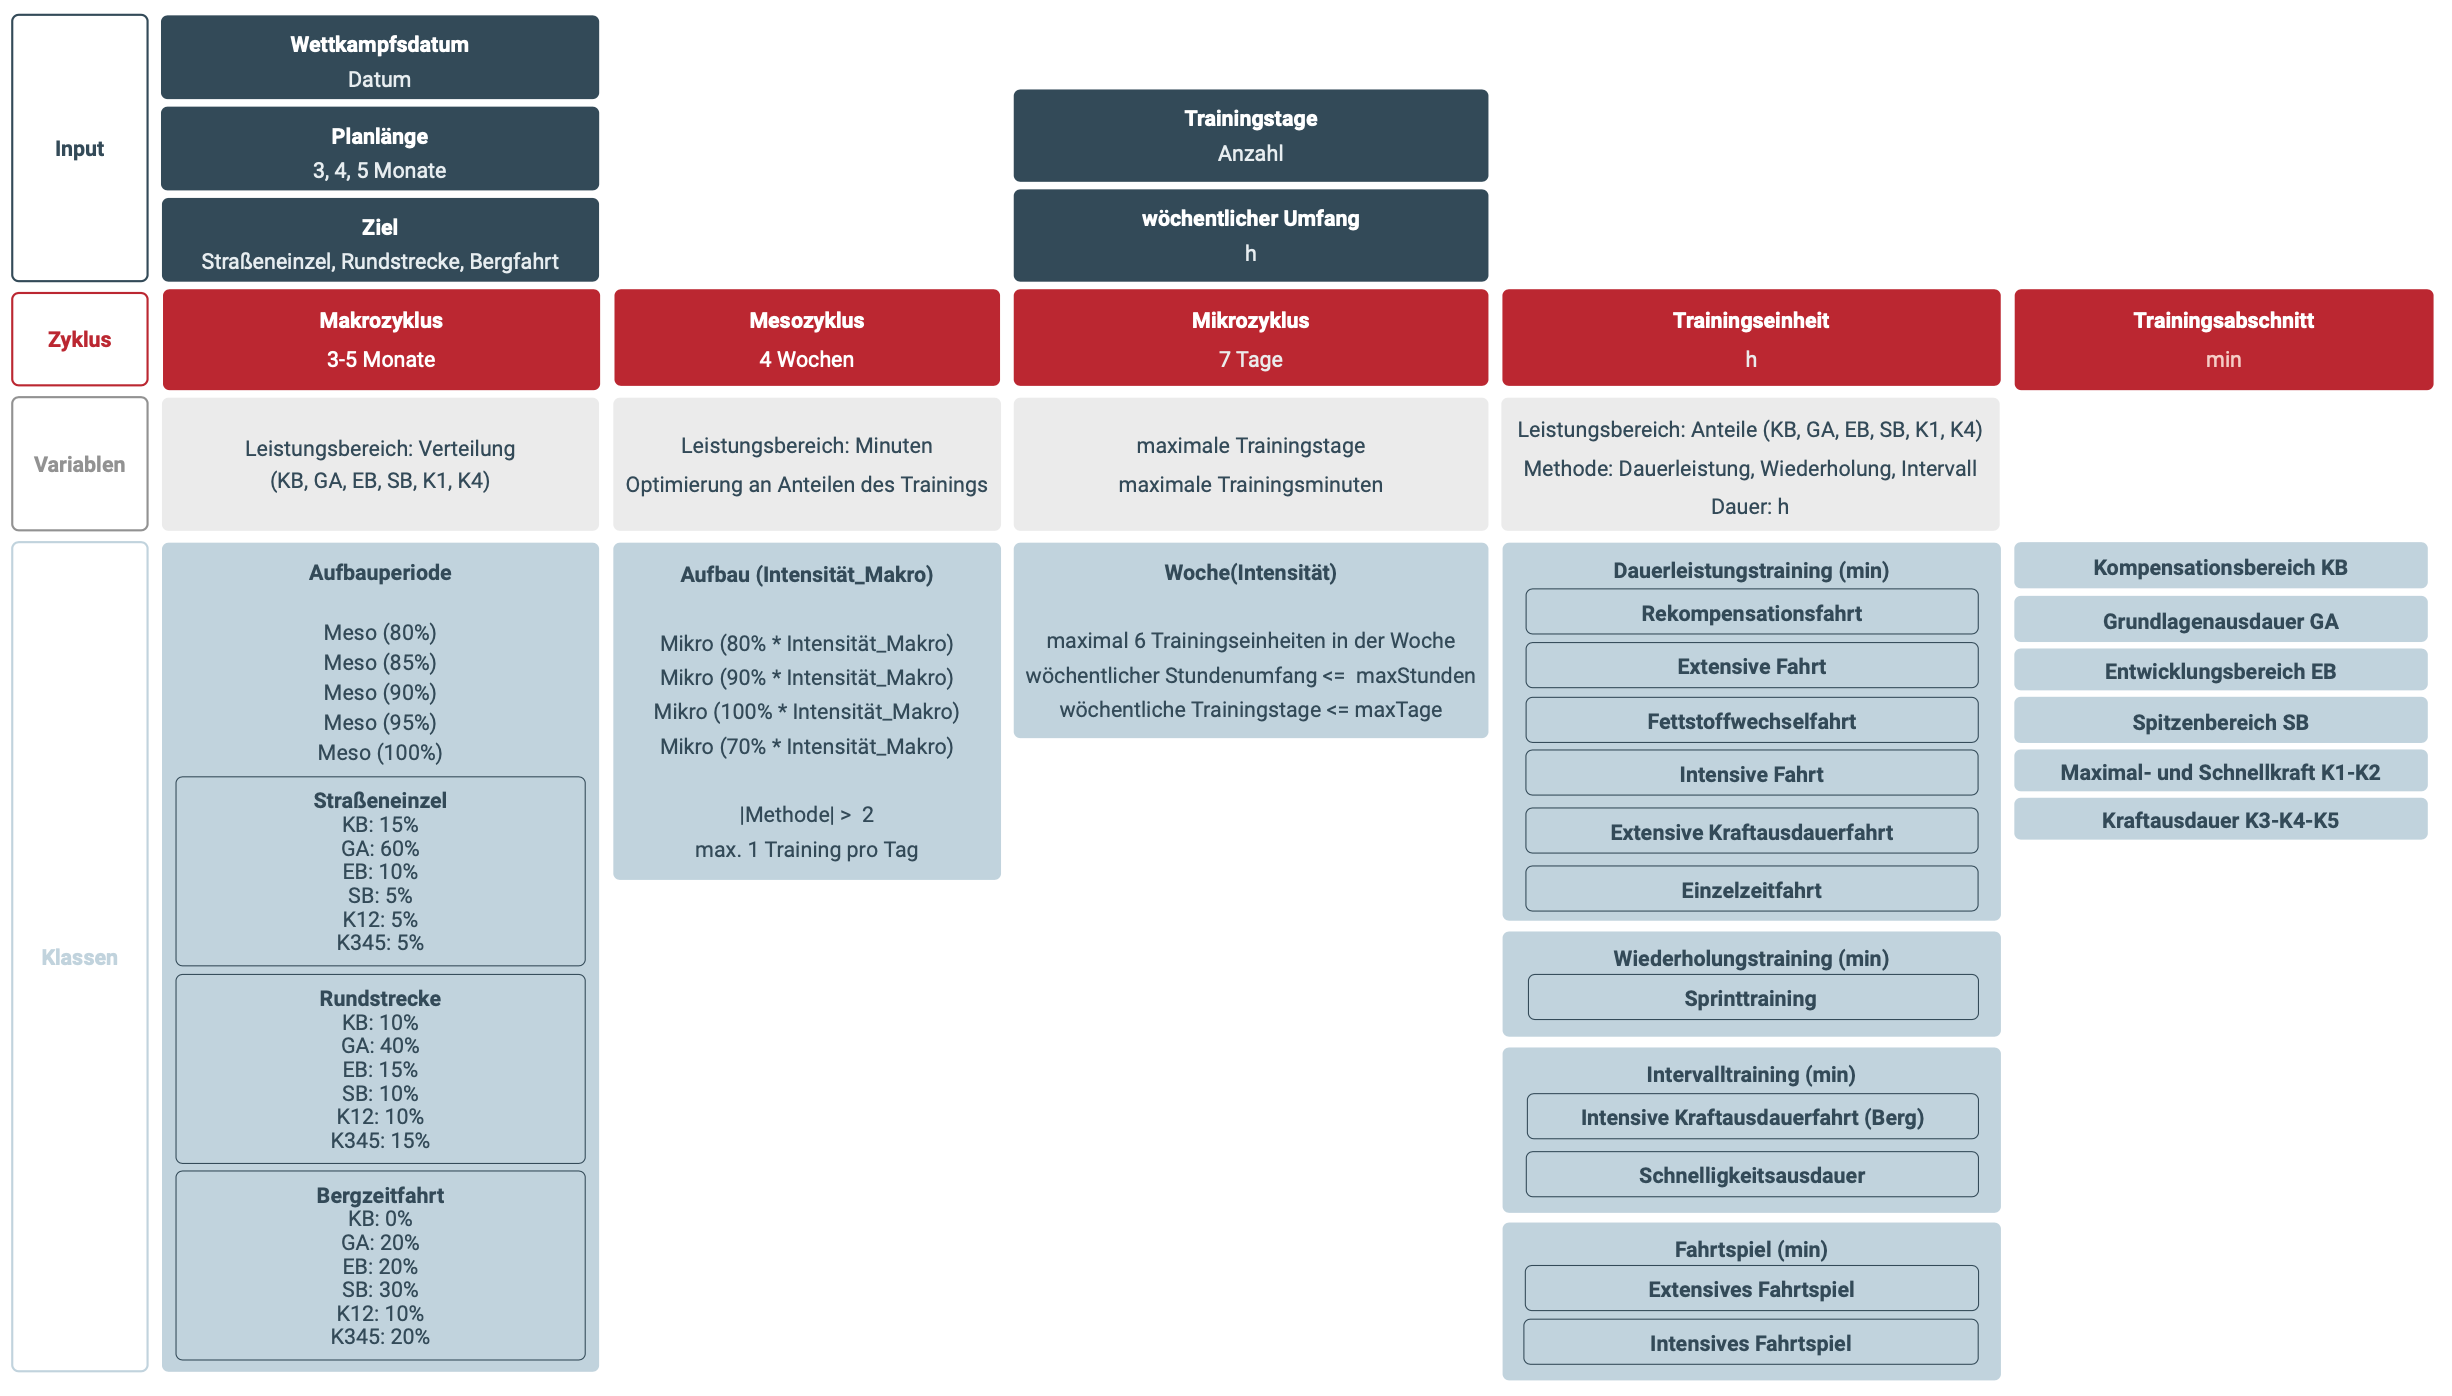
\includegraphics[width=\textwidth]{gfx/modellierung.png}
    \captionof{figure}{Schema der Modellierung}
    \end{minipage}
}

\newpage
\section{Trainingsplan im Freizeitsport}
\label{anhang:freizeitsport}

\newpage
\section{Trainingsplan im Amateursport}
\label{anhang:amateursport}
